\documentclass[10pt]{beamer}

\usepackage[style=british]{csquotes}
\usepackage{graphicx}

\usepackage{caption}
\usepackage{subcaption}
\usepackage{xcolor}
\usepackage[lined,boxed]{algorithm2e}



\usetheme[progressbar=frametitle]{metropolis}
\usepackage{appendixnumberbeamer}

\usepackage{booktabs}
\usepackage[scale=2]{ccicons}

\usepackage{pgfplots}
\usepgfplotslibrary{dateplot}

\usepackage{xspace}
\newcommand{\themename}{\textbf{\textsc{metropolis}}\xspace}

\title{A GAN Tutorial}
\subtitle{How GANs work and how to use them for speech technology research.}
% \date{\today}
\date{}
\author{Jacob Josiah Webber}
\institute{Centre for Speech Technology Research}
\titlegraphic{\hfill
\includegraphics[height=1.5cm]{logo.pdf}}

\begin{document}

\maketitle

\begin{frame}{Table of contents}
  \setbeamertemplate{section in toc}[sections numbered]
  \tableofcontents[hideallsubsections]
\end{frame}

\section{Introduction}

\begin{frame}[fragile]{Why are we here?}
%We present a new way of using neural networks to control speech.

In this talk I will
\begin{itemize}
    \item Describe GANs by
    \item defining \emph{generative} models
    \item Multimodal outputs
    \item showing how networks can be trained adversarially
    \item show some code examples
    \item and how to apply image modification techniques to speech
    \item and a recent paper from DeepMind on GAN TTS
\end{itemize}
\end{frame}

\begin{frame}{GANs (ideally) in Theory}
\begin{equation}
    \min_{\theta} \max_{\phi} V(G_\theta, D_\phi) = \mathbb{E}_{\mathbf{x} \sim \textbf{p}_{\textrm{data}}}[\log D_\phi(\textbf{x})] + 
\mathbb{E}_{\mathbf{z} \sim p(\textbf{z})}[\log (1-D_\phi(G_\theta(\textbf{z})))]
\end{equation}
(We'll come back to this)
\end{frame}

\begin{frame}{GANs in Practice}

\begin{figure}
    \centering
    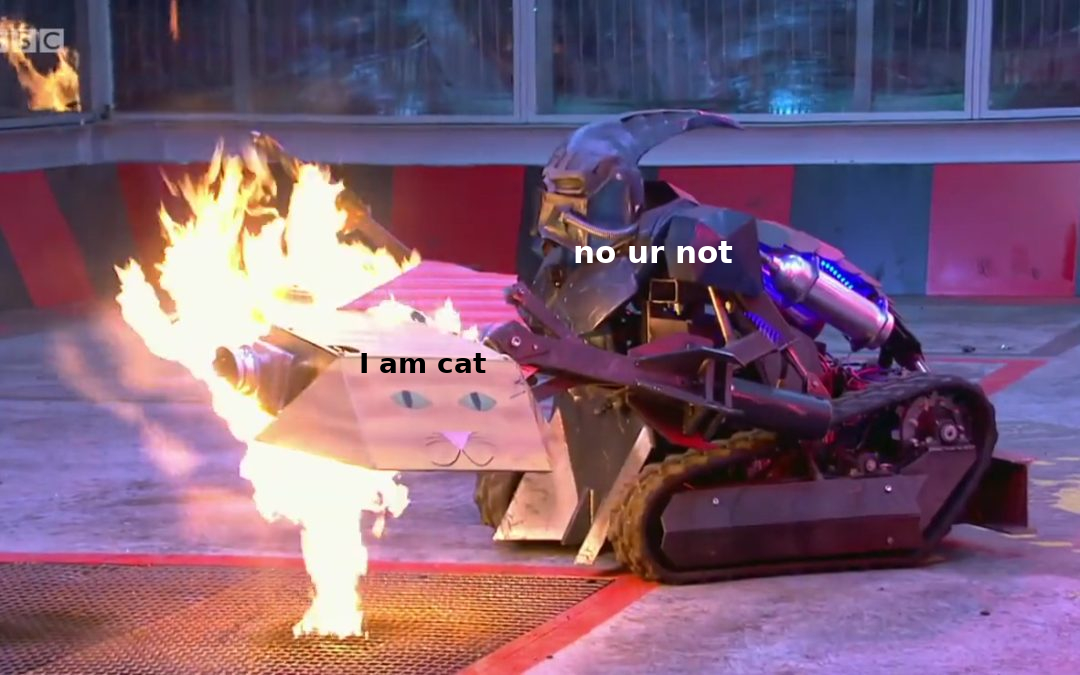
\includegraphics[width=0.94\textwidth]{figures/robot-wars.jpg}
    \caption*{Don't always work as planned...}
    \label{fig:robot-wars}
\end{figure}{}
\end{frame}{}

\section{Generative Models}

\begin{frame}{Generative models}

A statistical approach to generating samples

Take a training set, treating it as samples from a (unknown) distribution $p_{data}$

Using these samples (and some training algorithm and model) we estimate $p_{model}$

Sometimes this distribution only exists in theory, and the model only generates samples from it...

\end{frame}

\begin{frame}{Implicit vs. Explicit}

Models that generate a distribution that we sample from to get generate output can be described as \emph{explicit density} \cite{neurips} models (eg WaveRNN, WaveNet (FVBN))

Models that directly generate output (\emph{implicit density}) are generally used for GANs, because discriminator network needs real output to classify.

\end{frame}

\begin{frame}{Why GANs?}
    
\end{frame}{}

\section{How do GANs Work}

\begin{frame}{A Game Between Two Players}
Can be thought of as a game between two players...
\begin{itemize}
    \item We have Generator, $G$ and Discriminator $D$
    \item Discriminator is classifier between real/fake categories
    \item $D$ is trained on real images from the dataset
    \item $G$ is trained to maximise the realness estimated by $D$
\end{itemize}{}
    
\end{frame}

\begin{frame}{Adversarial?}
Why describe this as adversarial?

Each network optimises its \emph{own} parameters to minimise some cost that is at least partially defined by the output of the opponent network.    

Neither network can control the other's parameters to do this.

\end{frame}

\begin{frame}{What Is $G$?}
    How do you build a $G$?
    \begin{itemize}
        \item Use any differentiable function $G(z)$
        \item (A deep network)
        \item DCGAN: A deep convolutional net
        \item $z$ is some sort of seed -- can be random numbers, or can train a Adversarial system that takes some proper input.
    \end{itemize}{}
\end{frame}{}

\begin{frame}{The Training Process}
    
\IncMargin{1em}
\begin{algorithm}[H]
%\small
  \KwData{A dataset consisting of $N$ batches, $\mathbf{x}$}
  \KwResult{Trained network parameters}
  \ForEach{$\mathbf{x}$}{
%     \tcc{First train finder network}
%  	Generate hidden state by passing mel-spect into hider network\;
%  	Use finder network on hidden state to get estimated F0\;
%  	Calculate cross-entropy loss between estimated F0 and F0\;
%  	Backprop through finder parameters and update\;
%  	\tcc{Train hider and combiner}
%  	Pass F0 and hidden state into combiner\;
%  	Calculate MSE combiner loss and leakage loss, sum\;
%  	Backprop loss through \emph{both} hider \emph{and} combiner parameters\;
%  	Update combiner and hider parameters using Adam optimiser\;
  }
\caption{Training algorithm}
 % \label{alg:adv}
\end{algorithm}

\end{frame}{}

\begin{frame}{References}
\bibliographystyle{amsalpha}
    \bibliography{demo.bib}
\end{frame}{}

\end{document}
